\documentclass[a4paper,11pt]{article}
\usepackage{filecontents}

\usepackage[utf8]{inputenc}
\usepackage[english]{babel}
\usepackage{graphicx, array, blindtext}
\usepackage[colorinlistoftodos]{todonotes}
\DeclareUnicodeCharacter{2212}{-}
\usepackage [a4 paper , hmargin = 1.2 in , bottom = 1.5 in] {geometry}
\usepackage [parfill] {parskip}

\usepackage{enumitem}
\usepackage{amsmath}
\usepackage{amsthm}

\usepackage{nameref}
\usepackage{amssymb}
\usepackage [linesnumbered, ruled, vlined] {algorithm2e}
\usepackage{listings}
\usepackage{xcolor}
\usepackage{floatrow}
\usepackage{siunitx}
\usepackage{cancel}
\usepackage{fancyhdr}
\usepackage{graphicx}
\usepackage{verbatim}
\usepackage[document]{ragged2e}

\renewcommand{\footrulewidth}{0.4pt}
\newtheorem{definition}{Definition}
\numberwithin{definition}{section}
\newtheorem{mytheorem}{Theorem}
\numberwithin{mytheorem}{subsection}
\newcommand{\notimplies}{\;\not\!\!\!\longrightarrow}  
\newcommand\norm[1]{\left\lVert#1\right\rVert}
\pagestyle{fancy}
\fancyhf{}
\rhead{CS754 Assignment 2}
\lhead{200050013-200050130}
\fancyfoot[C]{Page \thepage}
\usepackage{subcaption}
\usepackage{listings}


\usepackage{hyperref}
\urlstyle{same}
\hypersetup{pdftitle={main.pdf},
    colorlinks=false,
    linkbordercolor=red
}
\usepackage{array}
\usepackage{listings,chngcntr}

\begin{document}
\centering{

\title{\fontsize{150}{60}{CS754 Assignment 2 Report}}

\author{
Arpon Basu \\ Shashwat Garg }
}

\date{Spring 2022}
\maketitle

\justifying
\tableofcontents

\newpage
\justifying
\section*{Introduction}

Welcome  to our report on CS754 Assignment 2. We have tried to make this report comprehensive and self-contained. We hope reading this would give you a proper flowing description of our work, methods used and the results obtained.


Hope you enjoy reading the report. Here we go!


\section{Problem 1}



\subsection{Given $\delta_{2s}=1$}

In this case, our RIP theorem inequality becomes-
$$0 \leq \norm{\Phi h}_2^2 \leq 2 \norm{h}_2^2$$
where $h$ is a 2s-sparse vector.

We know that $\delta_{2s}$ is the smallest number such that the above holds for all s-sparse vectors for the matrix $\Phi$.

This means that, unless the $\delta_{2s}=1$ is present to take care of the upper bound on $\norm{\Phi h}_2^2$, there will exist an s-sparse vector such that $\norm{\Phi h}_2^2=0$, which implies that $\Phi h =\boldsymbol{0}$. Denoting the columns of $\Phi$ as $C_1, C_2 \cdots C_n$ and the entries of $h$ as $a_1, a_2, \cdots a_n$, we can get that-
$$ \sum_{i=1}^n C_i \cdot a_i = 0 $$

If we focus only on the non-zero entries of $h$, we can get a linear combination of at-most 2s columns of $\Phi$ which sums up to 0. Thus, in this case, we can always say that 2s columns of $\Phi$ are linearly dependent.

Hence, when $\delta_{2s}=1$, 2s columns of $\Phi$ may be linearly dependent.

\subsection{Triangle Inequality}

We are trying to solve the following-

$$ \min_{\tilde{x} \in \mathbb{R}^n} \norm{\tilde{x}}_1 ~where ~\norm{y - \Phi \tilde{x}}_2 \leq \epsilon $$

The solution we receive is called $x^*$ and the actual, true, unknown solution is called $x$. Now, note that our reconstruction demands that  $\norm{y - \Phi x_{estimated}}_2 \leq \epsilon$

This implies that $x^*$ will also obey the same property.

Secondly, in the premise of the Theorem, we assume that the noise magnitude is less than $\epsilon$. This is one of the factors we take into account while choosing the $\epsilon$ value. Hence, by choice of $\epsilon$ in noise, we get that
$\norm{y - \Phi x}_2 \leq \epsilon$.

Finally, with these two tools, we can use the Triangle Inequality as follows-
$$\norm{\Phi(x^* - x)}_2 = \norm{(\Phi x^* - y) + (y - \Phi x)}_2 \leq \norm{\Phi x^* - y}_2 + \norm{y-\Phi x}_2$$
Using the two arguments above, we can say that-
$$\norm{\Phi x^* - y}_2 + \norm{y-\Phi x}_2 \leq \epsilon + \epsilon = 2\epsilon$$
Thus, finally, we get that 
$$\norm{\Phi(x^* - x)}_2 \leq \norm{\Phi x^* - y}_2 + \norm{y-\Phi x}_2 \leq 2\epsilon$$
Hence, proved.

\subsection{Relation between Norms}

We know that $l_\infty$ norm gives out the element with the maximum magnitude in the vector. Let us assume entries of $h_{T_j}$ to be $a_1, a_2, \cdots a_n$. WLOG, let us assume that, since $h_{T_j}$ is s-sparse, $a_1, a_2, \cdots a_s$ are non-zero and rest are 0. The re-ordering won't affect the solution since we would be taking the norm anyways.
With this knowledge, we can see that-
$$\forall a_i:i \leq s, (a_i)^2 \leq \norm{h_{T_j}}^2_\infty$$
Adding all these s inequalities up, since all $a_i$ for $i>s$ are zero, we get-
$$\norm{h_{T_j}}_2^2 \leq s \norm{h_{T_j}}_{\infty}^2$$
From this, we directly get that-
$$\norm{h_{T_j}}_2 \leq s^{1/2} \norm{h_{T_j}}_{\infty}$$

Secondly, by construction, we know that every element of $h_{T_j}$ is smaller than the every element of $h_{T_{j-1}}$. Thus, we can say the following-
$$\norm{h_{T_j}}_{\infty} \leq |b_i| $$
where $b_1, b_2, \cdots b_s$ are the s non-zero elements of $h_{T_{j-1}}$.
Adding these up for the s inequalities, and using the fact that all $b_i$ for $i>s$ are zero, we get-
$$s \norm{h_{T_j}}_\infty \leq \norm{h_{T_{j-1}}}_{1}$$
This is equivalent to-
$$s^{1/2} \norm{h_{T_j}}_\infty \leq  s^{-1/2} \norm{h_{T_{j-1}}}_{1}$$

Hence, finally, we have obtained the required relations-
$$\norm{h_{T_j}}_2 \leq s^{1/2} \norm{h_{T_j}}_\infty \leq  s^{-1/2} \norm{h_{T_{j-1}}}_1$$

\subsection{Summing up the norms}

By just summing up the above inequality, we can say that-
$$\norm{h_{T_j}}_2 \leq s^{-1/2} \norm{h_{T_{j-1}}}_1$$
$$\implies \sum \limits_{j \geq 2} \norm{h_{T_j}}_2 \leq s^{-1/2} \: (\norm{h_{T_1}}_1 + \norm{h_{T_2}}_1 + \ldots)$$

Also, we know that-
$$\norm{h_{T_0}}_1 + \norm{h_{T_1}}_1 + \norm{h_{T_2}}_1 + \ldots = \norm{h}_1$$
Thus, we can say that 
$$ \norm{h_{T_0^c}}_1 = \norm{h}_1 - \norm{h_{T_0}}_1 = \norm{h_{T_1}}_1 + \norm{h_{T_2}}_1 + \ldots $$ 

Hence, finally we have-

$$\sum \limits_{j \geq 2} \norm{h_{T_j}}_2 \leq s^{-1/2} ~(\norm{h_{T_1}}_1 + \norm{h_{T_2}}_1 + \ldots) \leq s^{-1/2}\norm{h_{T_0^c}}_1$$

\subsection{Extended Triangle Inequality}
\label{subsec1_5}

By definition of $h_{T_i}$, we can say that, $h_{(T_0 \cup T_1)^c} = \sum_{j \geq 2} h_{T_j}$
Thus, obviously
$$\norm{h_{(T_0 \cup T_1)^c}}_2 = \norm{\sum_{j \geq 2} h_{T_j}}_2$$
Also, from previous parts, we know that
$$\sum_{j \geq 2} \norm{h_{T_j}}_2 \leq s^{-1/2} \norm{h_{T_0^c}}_1$$

Now, by Triangle inequality, we know that-
$$\norm{h_{T_2} + h_{T_3} + \cdots}_2 \leq \norm{h_{T_2}}_2 + \norm{h_{T_2}}_2 + \cdots$$
This is equivalent to-
$$\norm{\sum_{j \geq 2} h_{T_j}}_2 \leq \sum_{j \geq 2} \norm{h_{T_j}}_2$$

Combining everything, we get-
$$\norm{h_{(T_0 \cup T_1)^c}}_2 = \norm{\sum_{j \geq 2} h_{T_j}}_2 \leq \sum_{j \geq 2} \norm{h_{T_j}}_2 \leq s^{-1/2} \norm{h_{T_0^c}}_1$$

\subsection{Reverse Triangle Inequality, for L1 norm}

Note that $x^*$ is the minimizer of the l1 norm. Thus, if we have chosen a correct error bound, we will get that-

$$\norm{x}_1 \geq \norm{x^*}_1 \implies \norm{x}_1 \geq \norm{x+h}_1$$
Now from reverse triangle inequality, I can say that, $\norm{a+b}_1 \geq \norm{a}_1 - \norm{b_1}$. Also I can split the L1-norm of (x+h) into terms in $T_0$ and those in $T_{0^c}$.

Thus finally, can say the following, by repeatedly applying triangle Inequality. Note that this is not the L2 norm inequality, but it works similarly, due to behaviour of the $||$ function. We are considering (x+h) to be (x-(-h)), while applying the inequality.
$$\sum \limits_{i \in T_0}|x_i + h_i| \geq \norm{x_{T_0}}_1 - \norm{h_{T_0}}_1$$
$$\sum \limits_{i \in T_0^c}|x_i + h_i| \geq \norm{h_{T_0^c}}_1 - \norm{x_{T_0^c}}_1 \footnote{(PS-Please note how the inequality was applied in the opposite sense)}$$

Adding these two, along with our previous results, we get-
$$ \norm{x}_1 \geq \norm{x+h}_1 = \sum \limits_{i \in T_0}|x_i + h_i| + \sum \limits_{i \in T_0^c}|x_i + h_i| \geq \norm{x_{T_0}}_1 - \norm{h_{T_0}}_1 + \norm{h_{T_0^c}}_1 - \norm{x_{T_0^c}}_1$$


\subsection{Rearranging}
\label{rearr}
Now, we have the following-
$$ \norm{x}_1 \geq \norm{x_{T_0}}_1 - \norm{h_{T_0}}_1 + \norm{h_{T_0^c}}_1 - \norm{x_{T_0^c}}_1$$
$$ \implies \norm{h_{T_0^c}}_1 \leq  \norm{h_{T_0}}_1 + \norm{x}_1 -\norm{x_{T_0}}_1 + \norm{x_{T_0^c}}_1 $$
Now, note that $x_{T_0^c} = x - x_{T_0}$. Thus, using triangle inequality, we can say that-
$$ \norm{x}_1 - \norm{x_{T_0}}_1 \leq \norm{x - x_{T_0}}_1 = \norm{x_{T_0^c}}_1$$

Combining the above two, we get-
$$ \norm{h_{T_0^c}}_1 \leq  \norm{h_{T_0}}_1 + \norm{x}_1 -\norm{x_{T_0}}_1 + \norm{x_{T_0^c}}_1 \leq  \norm{h_{T_0}}_1 + \norm{x_{T_0^c}}_1 + \norm{x_{T_0^c}}_1 = \norm{h_{T_0}}_1 + 2\norm{x_{T_0^c}}_1$$
Hence, proved.

\subsection{Using Cauchy-Schwartz}
\label{cauchy}
In section \ref{subsec1_5}, we have already seen the following result-
$$\norm{h_{(T_0 \cup T_1)^c}}_2 \leq s^{-1/2} \norm{h_{T_0^c}}_1$$
In the previous section, we saw the following-
$$ \norm{h_{T_0^c}}_1 \leq \norm{h_{T_0}}_1 + 2\norm{x_{T_0^c}}_1$$
Also, from the Cauchy-Schwartz inequality, we can say that the do product of two vectors is less than the product of their L2 norms. Thus, we can say that-

$$\norm{h_{T_0}}_1 \leq s^{1/2}\norm{h_{T_0}}_2$$

This is obtained by taking a signum function on $h_{T_0}$, which returns a vector with +1 in places where $h_{T_0}$ is positive and -1 in places where $h_{T_0}$ is negative. A dot product of the two, gives us the L1 norm on the LHS, and the other 2 L2 norms on the RHS. The inequality is the classic $\cos{x} \leq 1$

Finally, we can say that-
$$\norm{h_{(T_0 \cup T_1)^c}}_2 \leq s^{-1/2} \bigg(\norm{h_{T_0}}_1 + 2\,\norm{x_{T_0^c}}_1\bigg) \leq s^{-1/2} \bigg(s^{1/2} \norm{h_{T_0}}_2 + 2\norm{x_{T_0^c}}_1\bigg)$$
This is equivalent to the desired result, when $e_0 = s^{-1/2}\norm{x - x_s}_1$
$$\norm{h_{(T_0 \cup T_1)^c}}_2 \leq \norm{h_{T_0}}_2 + 2e_0$$

\subsection{Using RIP}
\label{rip}
We now use RIP for the first time in the proof. First, from definition of dot product or Cauchy-Schwartz inequality, we can say that-
$$\langle \Phi h_{T_0 \cup T_1}| \Phi h\rangle \leq \norm{\Phi h_{T_0 \cup T_1}}_2 \, \norm{\Phi h}_2$$
We will now put individual bounds on the two expressions.
Firstly, from RIP of order 2s, we can say that-
$$\norm{\Phi h_{T_0 \cup T_1}}_2 \leq (1 + \delta_{2s})^{1/2} \norm{ h_{T_0 \cup T_1}}_2$$
Next, we can say the following, using results derived above-
$$\norm{\Phi h}_2 = \norm{\Phi (x^* - x)}_2 \leq \norm{\Phi x^*}_2 + \norm{\Phi x}_2 \leq \epsilon + \epsilon = 2\epsilon$$

Combining the two, we get the following-
$$\langle \Phi h_{T_0 \cup T_1}| \Phi h\rangle \leq \norm{\Phi h_{T_0 \cup T_1}}_2 \norm{\Phi h}_2 \leq 2\epsilon(1 + \delta_{2s})^{1/2} \norm{ h_{T_0 \cup T_1}}_2 $$


\subsection{Using Lemma 2.1}
\label{lemma}
We are not giving the proof of Lemma 2.1 again. We will invoke it on $h_{T_0}$ and $h_{T_j}$. Both are s-sparse vectors by definition. Thus, we can apply the lemma directly to get the result. The lemma states-
$$\langle \Phi x| \Phi x' \rangle \leq \delta_{s + s'} \norm{x}_2 \norm{x'}_2$$
for all $x$ and $x'$ which are s-sparse.
We just plug in $x$ as $h_{T_0}$ and $x'$ as $h_{T_j}$, to get-
$$\langle \Phi h_{T_0}| \Phi h_{T_j}\rangle \leq \delta_{2s}\norm{h_{T_0}}_2 \norm{h_{T_j}}_2$$
Hence, proved.

\subsection{AM-GM Inequality}
\label{amgm}
Note that-
$$\norm{h_{T_0 \cup T_1}}^2_2 = \sum_{i \in T_0\cup T_1} {h_i}^2 = \sum_{i \in T_0} {h_i}^2 + \sum_{j \in T_1} {h_j}^2 = \norm{h_{T_1}}^2_2 + \norm{h_{T_0}}^2_2$$
Also, note that, from AM-GM inequality, we have that-
$$\frac{A+B}{2} \geq \sqrt{A\cdot B}$$
Substituting $A = \norm{h_{T_0}}^2_2$ and $B = \norm{h_{T_1}}^2_2$, we get that-
$$\frac{\norm{h_{T_0}}^2_2+\norm{h_{T_1}}^2_2}{2} \geq \sqrt{\norm{h_{T_0}}^2_2\cdot \norm{h_{T_1}}^2_2}$$
Finally, we can say that-
$$\norm{h_{T_0 \cup T_1}}^2_2 = \frac{\norm{h_{T_0}}^2_2}{2}  + \frac{\norm{h_{T_1}}^2_2}{2}  + \frac{\norm{h_{T_0}}^2_2}{2} + \frac{\norm{h_{T_1}}^2_2}{2} \geq \frac{\norm{h_{T_1}}^2_2}{2} + \frac{\norm{h_{T_0}}^2_2}{2} + \sqrt{\norm{h_{T_0}}^2_2\cdot \norm{h_{T_1}}^2_2}$$
We can write the same as-
$$2 \cdot \norm{h_{T_0 \cup T_1}}^2_2 \geq (\norm{h_{T_0}}_2 + \norm{h_{T_1}}_2)^{2}$$
Taking the square-root, we have-
$$\sqrt{2} \cdot \norm{h_{T_0 \cup T_1}}_2 \geq \norm{h_{T_0}}_2 + \norm{h_{T_1}}_2$$

Hence, shown.

\subsection{Bounding norm of \textbf{h}}

Firstly, from the RIP property, we have-
From the restricted isometry property, we have
$$(1 - \delta_{2s}) \norm{h_{T_0 \cup T_1}}_2^2 \leq \norm{\Phi h_{T_0 \cup T_1}}_2^2$$

For the second part, we need some more results. Note that we can use the Triangle Inequalities, \ref{lemma} and \ref{amgm} to show the following-
$$\langle \Phi h_{T_0} + \Phi h_{T_1}| \Phi h_{T_j}\rangle \leq \langle \Phi h_{T_0}| \Phi h_{T_j}\rangle + \langle \Phi h_{T_1}| \Phi h_{T_j}\rangle$$
$$\langle \Phi h_{T_0}| \Phi h_{T_j}\rangle + \langle \Phi h_{T_1}| \Phi h_{T_j}\rangle \leq \delta_{2s} (\norm{h_{T_0}}_2 + \norm{h_{T_1}}_2) \norm{h_{T_{j}}} \leq  \delta_{2s} \sqrt{2}\,\norm{h_{T_0 \cup T_1}} \norm{h_{T_{j}}}$$
Combining the two inequalities above and adding the over j-index.
$$\langle \Phi h_{T_0} + \Phi h_{T_1}| \sum_{j \geq 2} \Phi h_{T_j}\rangle \leq \delta_{2s} \sqrt{2} \norm{h_{T_0 \cup T_1}}(\sum \limits_{j \geq 2} \norm{h_{T_j}}_2)$$
$$\implies \langle \Phi h_{T_0 \cup T_1}| \sum_{j \geq 2} \Phi h_{T_j}\rangle \leq \delta_{2s} \sqrt{2} \norm{h_{T_0 \cup T_1}}(\sum \limits_{j \geq 2} \norm{h_{T_j}}_2)$$
Using \ref{rip}, we can invoke the following-
$$\langle \Phi h_{T_0 \cup T_1}| \Phi h\rangle \leq (1 + \delta_{2s})^{1/2} \norm{ h_{T_0 \cup T_1}}_2 $$
which is the same as-
$$\langle \Phi h_{T_0 \cup T_1}|  \Phi h_{T_0 \cup T_1} + \sum_{j \geq 2} \Phi h_{T_j} \rangle \leq 2\epsilon(1 + \delta_{2s})^{1/2} \norm{ h_{T_0 \cup T_1}}_2 $$
Invoking the triangle inequality, I can say that-
$$\langle \Phi h_{T_0 \cup T_1}| \Phi h_{T_0 \cup T_1} \rangle \leq \langle \Phi h_{T_0 \cup T_1}| \sum_{j \geq 2} \Phi h_{T_j}\rangle + \langle \Phi h_{T_0 \cup T_1}|  \Phi h_{T_0 \cup T_1} + \sum_{j \geq 2} \Phi h_{T_j} \rangle$$
Thus, using the two inequalities derived above, we get that-
$$\langle \Phi h_{T_0 \cup T_1}| \Phi h_{T_0 \cup T_1} \rangle \leq  2\epsilon(1 + \delta_{2s})^{1/2} \norm{ h_{T_0 \cup T_1}}_2 + \delta_{2s} \sqrt{2} \norm{h_{T_0 \cup T_1}}(\sum \limits_{j \geq 2} \norm{h_{T_j}}_2)$$
Thus, we finally have the following-
$$(1 - \delta_{2s}) \norm{h_{T_0 \cup T_1}}_2^2 \leq \norm{\Phi h_{T_0 \cup T_1}}_2^2 \leq \norm{ h_{T_0 \cup T_1}}_2 (2\epsilon (1 + \delta_{2s})^{1/2} + \delta_{2s}\sqrt{2}\sum \limits_{j \geq 2} \norm{h_{T_j}}_2) $$

Hence, justified.

\subsection{Rearranging (again)}
\label{rearr2}
Let us remind ourselves of the following from \ref{subsec1_5}-
$$\sum_{j \geq 2} \norm{h_{T_j}}_2 \leq s^{-1/2} \norm{h_{T_0^c}}_1$$

The previous inequality said that-
$$(1 - \delta_{2s}) \norm{h_{T_0 \cup T_1}}_2^2 \leq \norm{ h_{T_0 \cup T_1}}_2 (2\epsilon (1 + \delta_{2s})^{1/2} + \delta_{2s}\sqrt{2}\sum \limits_{j \geq 2} \norm{h_{T_j}}_2) $$

Combining the two above, we get that-
$$(1 - \delta_{2s}) \norm{h_{T_0 \cup T_1}}_2^2 \leq \norm{ h_{T_0 \cup T_1}}_2 (2\epsilon (1 + \delta_{2s})^{1/2} + \delta_{2s}\sqrt{2}s^{-1/2} \norm{h_{T_0^c}}_1) $$

Removing a factor of $\norm{h_{T_0 \cup T_1}}_2^2$, we get-
$$(1 - \delta_{2s}) \norm{h_{T_0 \cup T_1}}_2 \leq 2\epsilon (1 + \delta_{2s})^{1/2} + \delta_{2s}\sqrt{2}s^{-1/2} \norm{h_{T_0^c}}_1 $$
which is the same as-
$$ \norm{h_{T_0 \cup T_1}}_2 \leq  \alpha\epsilon + p s^{-1/2} \norm{h_{T_0^c}}_1 $$
where, $\alpha = \frac{2 \sqrt{1 + \delta_{2s}}}{1 - \delta_{2s}}$ and $p = \frac{\sqrt{2}\delta_{2s}}{1 - \delta_{2s}}$. Hence shown.

\subsection{Condensing the inequalities}

From \ref{rearr}, we know that-
$$ \norm{h_{T_0^c}}_1 \leq  \norm{h_{T_0}}_1 + 2\norm{x_{T_0^c}}_1$$
Using this in the above inequality, we can say-
$$ \norm{h_{T_0 \cup T_1}}_2 \leq  \alpha\epsilon + p s^{-1/2} \norm{h_{T_0^c}}_1 \leq \alpha\epsilon + p s^{-1/2}\norm{h_{T_0}}_1 + 2p s^{-1/2}\norm{x_{T_0^c}}_1$$
Now, using triangle inequality and Cauchy-Schwartz, like a lot of times before-
$$ s^{-1/2} \norm{h_{T_0}}_1 \leq \norm{h_{T_0}}_2 \leq \norm{h_{T_0 \cup T_1}}_2$$
This gives us-
$$ \norm{h_{T_0 \cup T_1}}_2 \leq \alpha\epsilon + p \norm{h_{T_0 \cup T_1}}_2 + 2p e_0$$
where, $e_0 = s^{-1/2}\norm{x_{T_0^c}}_1$

This can be easily rearranged to give-
$$ \norm{h_{T_0 \cup T_1}}_2 \leq (1-p)^{-1}(\alpha\epsilon + 2p e_0)$$

\subsection{Bringing it all together}

By Triangle Inequality, we have that-
$$\norm{h}_2 \leq \norm{h_{T_0 \cup T_1}}_2 + \norm{h_{(T_0 \cup T_1)^c}}_2$$

From \ref{cauchy}, we know that-
$$\norm{h_{(T_0 \cup T_1)^c}}_2 \leq \norm{h_{T_0}}_2 + 2e_0 \leq \norm{h_{T_0\cup T_1}}_2 + 2e_0$$

This gives-
$$\norm{h}_2 \leq \norm{h_{T_0 \cup T_1}}_2 + \norm{h_{(T_0 \cup T_1)^c}}_2 \leq \norm{h_{T_0\cup T_1}}_2 + \norm{h_{T_0\cup T_1}}_2 + 2e_0 \leq 2\norm{h_{T_0\cup T_1}}_2 + 2e_0$$

Using the previous inequality, we have-
$$ \norm{h_{T_0 \cup T_1}}_2 \leq (1-p)^{-1}(\alpha\epsilon + 2p e_0)$$

Substituting $\norm{h_{T_0 \cup T_1}}_2$ from above, we have-
$$\norm{h}_2 \leq \norm{h_{T_0 \cup T_1}}_2 + \norm{h_{(T_0 \cup T_1)^c}}_2 \leq 2\norm{h_{T_0\cup T_1}}_2 + 2e_0 \leq (1-p)^{-1}(\alpha\epsilon + 2p e_0) + 2\epsilon$$

And now, finally after simplifying, we get-
$$\norm{h}_2 \leq \norm{h_{T_0 \cup T_1}}_2 + \norm{h_{(T_0 \cup T_1)^c}}_2 \leq 2\norm{h_{T_0\cup T_1}}_2 + 2e_0 \leq 2(1-p)^{-1}(\alpha\epsilon + (1+p) e_0)$$

which is what we needed to show.

\subsection{Wrapping up}

By Definition, we can say that-
$$\norm{h}_1 = \norm{h_{T_0}}_1 + \norm{h_{T_0^c}}_1$$

Now, from our long journey of proving inequations, we can state the following-
$$\norm{h_{T_0}}_1 \leq s^{1/2}\norm{h_{T_0}}_2 \leq s^{1/2}\norm{h_{T_0\cup T_1}}_2$$
Since we have been given that $h$ is in the nullspace of $\Phi$, this means that error $\epsilon = 0$, as the case is noiseless.

Hence, from \ref{rearr2}, we can say that, with $\epsilon = 0$-
$$\norm{h_{T_0 \cup T_1}}_2 \leq p s^{-1/2} \norm{h_{T_0^c}}_1$$
$$\implies s^{1/2}\norm{h_{T_0 \cup T_1}}_2 \leq p \norm{h_{T_0^c}}_1$$

This gives-
$$\norm{h_{T_0}}_1 \leq s^{1/2}\norm{h_{T_0\cup T_1}}_2 \leq p \norm{h_{T_0^c}}_1$$

Finally-
$$\norm{h}_1 = \norm{h_{T_0}}_1 + \norm{h_{T_0^c}}_1 \leq \norm{h_{T_0^c}}_1 + p \norm{h_{T_0^c}}_1 = (1 + p)\norm{h_{T_0^c}}_1$$

From \ref{rearr}, we can get that-
$$ \norm{h_{T_0^c}}_1 \leq \norm{h_{T_0}}_1 + 2\norm{x_{T_0^c}}_1 \leq p \norm{h_{T_0^c}}_1 + 2\norm{x_{T_0^c}}_1$$
$$\implies \norm{h_{T_0^c}}_1 \leq 2(1-p)^{-1} \norm{x_{T_0^c}}_1$$

Combining all, we get-
$$\norm{h}_1 = \norm{h_{T_0}}_1 + \norm{h_{T_0^c}}_1 \leq 2(1+p)(1-p)^{-1} \norm{x_{T_0^c}}_1$$

And for the last time,\\
Hence, proved.





\section{Problem 2}
(a) First of all, note that $\boldsymbol{\Phi x = \Phi_S\widetilde{x}}$, since all other entries of $\boldsymbol{x}$ are zero, and hence all the corresponding columns of $\boldsymbol{\Phi}$ get nullified.

Now, we introduce the notion of \textbf{pseudo-inverse} as mentioned in the question: For any matrix $A$ (which can be rectangular too), there exists a unique \textbf{Moore-Penrose pseudo-inverse} $\boldsymbol{A^{\dagger}}$ which mimics many of the properties that the actual inverse satisfies. In particular, if it so happens that the columns of $A$ are linearly independent, then $A^{\dagger}A = I$.

Also note that since we are assuming $\boldsymbol{\Phi}$ satisfies RIC of order $S$, it automatically implies that any $S$ columns of $\boldsymbol{\Phi}$ are linearly independent. Thus hereon we can assume WLOG that $\boldsymbol{\Phi^{\dagger}_S\Phi_S = I}$.

Armed with this knowledge, it's very easy to determine the oracular solution: Note that while deriving any \textbf{deterministic} theoretical solution, we must ignore the noise $\boldsymbol{\eta}$ as we have no precise way of quantifying it apart from an upper bound on it's norm. Thus, $\boldsymbol{y_{\mathrm{theoretical}} = \Phi x = \Phi_s \widetilde{x}}$, and thus 
$$\boldsymbol{\widetilde{x} = \Phi_S^{\dagger}y_{\mathrm{theoretical}}}$$
Note that we don't actually know the value of $\boldsymbol{y_{\mathrm{theoretical}}}$. This is a shortcoming that is fixed below.

(b) Clearly 
\begin{gather*}
\boldsymbol{y = \Phi x + \eta = \Phi_S\widetilde{x} + \eta} \\
\Rightarrow \boldsymbol{\Phi^{\dagger}_S y = \Phi_S^{\dagger}\Phi_S \widetilde{x} + \Phi_S^{\dagger}\eta = \widetilde{x} + \Phi_S^{\dagger}\eta}
\end{gather*}
Treating $\boldsymbol{\Phi^{\dagger}_S y}$ as the ``actual" $\boldsymbol{x}$, we get that 
\begin{gather*}
    \boldsymbol{x = \widetilde{x} + \Phi^{\dagger}_S\eta}\\
    \Rightarrow\boldsymbol{\lVert x-\widetilde{x}\rVert_2 = \lVert\Phi_S^{\dagger}\eta\rVert_2 }
\end{gather*}
Now, from the theory of \textbf{Singular Value Decomposition} we recall that the largest singular value of any matrix $A$ could be framed as the maximum of the following optimization problem
$$\boldsymbol{\sigma_{\mathrm{max}} = \lVert A\rVert_2 = \mathrm{max}_{\lVert x\rVert_2 = 1}\lVert Ax\rVert_2}$$
Then it's a direct consequence of the above maximization that $\boldsymbol{\lVert\Phi_S^{\dagger}\eta\rVert_2 \leq \lVert\Phi_S^{\dagger}\rVert_2\lVert\eta\rVert_2}$, as desired.

(c) We first prove a short lemma:

\textbf{Lemma: } Let $\boldsymbol{A}$ be any matrix. Then the non zero singular values of $\boldsymbol{A^{\dagger}}$ are the reciprocals of the non zero singular values of $\boldsymbol{A}$.

\textbf{Proof: } Let $\boldsymbol{A = U\Sigma V^*}$ be the SVD of $\boldsymbol{A}$. Then 
$$\boldsymbol{A^{\dagger} = (A^*A)^{-1}A^* = ((V\Sigma^*U^*)U\Sigma V^*)^{-1}(V\Sigma^*U^*) = V(\Sigma^*\Sigma)^{-1}\Sigma^*U^* = V\Sigma^{\dagger}U^*}$$
since $\boldsymbol{U}$ and $\boldsymbol{V}$ being unitary matrices satisfy the property that $\boldsymbol{U^* = U^{-1}}$ and $\boldsymbol{V^* = V^{-1}}$.

Now, from the properties of SVD we know that $\boldsymbol{\Sigma}$ is a rectangular matrix whose diagonal entries contain the singular values of $\boldsymbol{A}$.

Also, by the properties of the pseudo-inverse, one can obtain that the pseudo-inverse of $\boldsymbol{\Sigma}$ is obtained in a similar way in which we invert a diagonal matrix, ie: Take all the non zero entries of $\boldsymbol{\Sigma}$ (which occur in the diagonal), take their reciprocals, and finally take the transpose of the matrix that is obtained (the transpose is a consequence of the pseudo-inverse: The pseudo-inverse of a rectangular matrix has the dimensions of its transpose).

But then by the above derivation we also saw that the singular values of $\boldsymbol{A^{\dagger}}$ were basically the diagonal entries of $\boldsymbol{\Sigma^{\dagger}}$.

Thus, we obtain that the (non zero) singular values of $\boldsymbol{\Phi_S^{\dagger}}$ are the reciprocals of the singular values of $\boldsymbol{\Phi_S}$ (just plugin $\boldsymbol{A = \Phi_S}$ in the previous paragraph).

Also note that for any matrix $A$, it's singular values are the square roots of the eigenvalues of $\boldsymbol{AA^*}$, and thus the singular values of $\boldsymbol{A^{\dagger}}$ are the square roots of the reciprocals of the eigenvalues of $\boldsymbol{AA^*}\;$\footnote{note that the eigenvalues of $\boldsymbol{AA^*}$ are non-negative by the Spectral theorem since $\boldsymbol{AA^*}$ is Hermitian}.

Now, since $\boldsymbol{\Phi}$ is RIC with order $|S| = 2k$, from the slides (\texttt{CS\_Theory, Pg.101/109}) we have that $\boldsymbol{\delta_{2k}}$ = max$\boldsymbol{(\lambda_{\mathrm{max}}-1, 1-\lambda_{\mathrm{min}})}$ where $\boldsymbol{\lambda_{\mathrm{max}}}$ is the maximum eigenvalue of $\boldsymbol{\Phi_{\Gamma}\Phi_{\Gamma}^*}$ and $\boldsymbol{\lambda_{\mathrm{min}}}$ is the minimum eigenvalue of $\boldsymbol{\Phi_{\Gamma}\Phi_{\Gamma}^*}$ over all possible sets $\boldsymbol{\Gamma\subseteq[n],\;|\Gamma| \leq |S|}$ (note that $\boldsymbol{\lambda_{\mathrm{max}}}$ and $\boldsymbol{\lambda_{\mathrm{min}}}$ both don't necessarily come from some same set $\boldsymbol{\Gamma}$). 

Then, considering the fact that $\boldsymbol{\Phi_{\Gamma}\Phi_{\Gamma}^*}$ and $\boldsymbol{\Phi_{\Gamma}^*\Phi_{\Gamma}}$ have the same non-zero eigenvalues \footnote{this is again a linear algebra property: For any matrix $A$, $\boldsymbol{AA^*}$ and $\boldsymbol{A^*A}$ have the same non zero eigenvalues}, we see that every eigenvalue of $\boldsymbol{\Phi_S^*\Phi_S}$ lies in $\boldsymbol{[1-\delta_{2k}, 1+\delta_{2k}]}$ (because note that $S$ is just an instance of $\boldsymbol{\Gamma}$ and  $\boldsymbol{\delta_{2k}}$ = max$\boldsymbol{(\lambda_{\mathrm{max}}-1, 1-\lambda_{\mathrm{min}})}$ implies that all eigenvalues, are first bounded by $\boldsymbol{\lambda_{\mathrm{max}}}$ and $\boldsymbol{\lambda_{\mathrm{min}}}$ which are in turn bounded by $\boldsymbol{1-\delta_{2k}}$ and $\boldsymbol{1+\delta_{2k}}$.

Refer to the solution of Q3 for an elaboration of the same), and consequently \textbf{EVERY} singular value of $\boldsymbol{\Phi_S^{\dagger}}$, which as we showed above were the square roots of the reciprocals of the eigenvalues of $\boldsymbol{\Phi_S^*\Phi_S}$, must lie within $\boldsymbol{[\frac{1}{\sqrt{1+\delta_{2k}}}, \frac{1}{\sqrt{1-\delta_{2k}}}]}$, as desired.

(d) Note that Thm. 3 said that $\boldsymbol{\lVert x^* - x\rVert_2\leq\frac{C_0}{\sqrt{S}}\lVert x-\widetilde{x}\rVert_2 + C_1\epsilon}$. But we already know that $\boldsymbol{\lVert x-\widetilde{x}\rVert_2\leq\frac{\epsilon}{\sqrt{1-\delta_{2k}}}\leq\frac{\epsilon}{\sqrt{2-\sqrt{2}}}}$, since $\boldsymbol{\delta_{2k} \leq \sqrt{2} - 1}$ for Thm. 3 to hold.

Thus, $\boldsymbol{\lVert x^* - x\rVert_2\leq(\frac{C_0}{\sqrt{(2-\sqrt{2})S}} + C_1)\epsilon}$, and since $C_0$ and $C_1$ are known bounded constants we obtain that (the errors in) both the solutions are some constant factors of $\boldsymbol{\epsilon}$, and consequently some constant factors of each other.




\section{Problem 3}
We establish a certain lemma first before proving the asked for result.

\subsection{The Submatrix Lemma}
\textbf{Claim: } Let $\boldsymbol{A \in \mathbb{K}^{m\times n}}$ be a matrix and let $\boldsymbol{A_s \in \mathbb{K}^{m\times s}}$ be a submatrix of $\boldsymbol{A}$. Then all the eigenvalues of $\boldsymbol{A_s^{*}A_s}$ are also eigenvalues of $\boldsymbol{A^{*}A}$.

\textbf{Proof: } Notice that the sampling of $\boldsymbol{A_s}$ from $\boldsymbol{A}$ can be done via a \textbf{selection matrix} $\boldsymbol{B\in\mathbb{K}^{n\times s}}$ such that $\boldsymbol{A_s = AB}$. Notice that the columns of $\boldsymbol{B}$ are just ``one-hot" columns corresponding to the columns of $\boldsymbol{A}$ which were sampled to make $\boldsymbol{A_s}$. One of the consequences of this is that $\boldsymbol{BB^* = I_n \in \mathbb{K}^{n\times n}}$. We shall use this below.

Also, WLOG assume that $\boldsymbol{A_s}$ are the first $s$ columns of $\boldsymbol{A}$ (if not, then we can always swap columns without affecting ``global" matrix properties such as eigenvalues).

Then, note that 
\begin{gather*}
    \boldsymbol{A_s^*A_sx = \lambda x},\;\mathrm{where}\;x\neq 0\;\mathrm{is}\;\mathrm{an}\;\mathrm{eigenvector}\;\mathrm{of}\;A_s^*A_s \\
    \Rightarrow \boldsymbol{(AB)^*(AB)x = \lambda x} \\
    \Rightarrow \boldsymbol{B^*A^*ABx = \lambda x} \\
    \Rightarrow \boldsymbol{BB^*A^*ABx = \lambda Bx} \\
    \Rightarrow \boldsymbol{A^*A(Bx) = \lambda (Bx)}
\end{gather*}

Thus, if $\boldsymbol{Bx \neq 0}$, then $\boldsymbol{\lambda}$ is an eigenvalue of $\boldsymbol{A^*A}$ with eigenvector $\boldsymbol{Bx}$. But note that (since we assumed that $\boldsymbol{A_s}$ comprised of the first $s$ columns of $\boldsymbol{A}$) $\boldsymbol{B}$ is basically $\boldsymbol{I_s}$ padded below with $(n-s)$ zero row vectors, and consequently $\boldsymbol{Bx}$ = $[\boldsymbol{x}^T\;\boldsymbol{0}^T_{n-s}]^T$, where $\boldsymbol{0}_{n-s}\in\mathbb{K}^{n-s}$ is the zero vector.

Since $\boldsymbol{x\neq 0}$, $\boldsymbol{Bx}$, whose first $s$ entries are identical to $\boldsymbol{x}$'s, can't be zero either, and consequently $\boldsymbol{Bx}$ is a valid eigenvector for $\boldsymbol{A^*A}$ and hence $\boldsymbol{\lambda}$ is an eigenvalue of $\boldsymbol{A^*A}$.

But now we're almost done: As in Q2, we can say that $\boldsymbol{\delta_{s}}$ = max$\boldsymbol{(\lambda_{\mathrm{max}}-1, 1-\lambda_{\mathrm{min}})}$ implying that every non-zero eigenvalue of $\boldsymbol{\Phi_{\Gamma}^*\Phi_{\Gamma}}$ ($\boldsymbol{|\Gamma| = s}$) \footnote{once again, CS Theory actually talks of the eigenvalues of $\boldsymbol{\Phi_{\Gamma}\Phi_{\Gamma}^*}$, but since we know that the non-zero eigenvalues of $\boldsymbol{\Phi_{\Gamma}^*\Phi_{\Gamma}}$ and $\boldsymbol{\Phi_{\Gamma}\Phi_{\Gamma}^*}$ are the same, we swap the $*$ according to our wishes} for any $s$ column sampling of $\boldsymbol{\Phi}$ must lie within $\boldsymbol{[1-\delta_s, 1+\delta_s]}$.

In particular, for some $s$-sampling, either the largest eigenvalue of $\boldsymbol{\Phi_{\Gamma}^*\Phi_{\Gamma}}$ is $\boldsymbol{(1+\delta_s)}$ or the smallest eigenvalue is $\boldsymbol{(1-\delta_s)}$. In either case, take that $\boldsymbol{\Phi_{\Gamma}}$ and append any $(t-s)$ new columns of $\boldsymbol{\Phi}$ to it.

For the resulting $m\times t$ matrix, by the submatrix lemma we have that it either has $\boldsymbol{(1+\delta_s)}$ or $\boldsymbol{(1-\delta_s)}$ as it's eigenvalue, and once again by the RIC property (that all eigenvalues are bounded by $(1\pm \delta)$), we either have that $\boldsymbol{(1-\delta_s) \geq (1-\delta_t)}$ or $\boldsymbol{(1+\delta_s) \leq (1+\delta_t)}$, both of which yield $\boldsymbol{\delta_s\leq\delta_t}$, as desired.


\section{Problem 4}

\begin{center}
    \begin{tabular}{ |p{3.5cm}||p{10cm}|}
   
    \hline
    \multicolumn{2}{|c|}{Paper Details} \\
    \hline
    Title of the Paper& Coded Aperture Design in Compressive Spectral Imaging
    Based on Side Information \\
    \hline
    Link of the paper  &  \href{https://opg.optica.org/viewmedia.cfm?uri=ao-56-22-6332&seq=0&am=y}{\textbf{Click Here}}  \\
    \hline
    Author List & Laura Galvis, Daniel Lau, Xu Ma, Henry Arguello, and Gonzalo R. Arce \\
    \hline
    Publication Date   &  July 2017 \\
    \hline
    Publication Venue  & Applied Optics 56, 6332-6340, The Optical Society 2017 \\
    \hline
    
    
   \end{tabular}
\end{center}

\subsection{Imaging System}
This paper proposes a method to use side information from an RGB sensor to design the coded-aperture patterns of a CSI imager. This is done in a way such that the high frequencies are promoted, leading to more detailed reconstructed spectral images. This means that the coded apertures are designed to follow the spatial structure such that more detailed spatial images and wavelength profiles can be reconstructed.

Basically, the side information is used as input of an edge detection algorithm to approximate a version of the edges of the spectral images. 
\begin{center}
    \begin{figure}[!h]
        \includegraphics[width=300px]{"imaging_system.png"}
    \end{figure}
\end{center}

The base is the CASSI camera, which captures 2D projections of the scene using a coded-snapshot. A beam splitter is used to divide the incident light into the two optical paths, the CASSI and the RGB arms. The RGB arm also simultaneously captures the image information. The RGB arm is not only used for sensing, but also to achieve super-resolution during reconstruction. We'll elaborate how soon.



\subsection{ Designing the Coded Aperture}

Bernoulli matrices are usually used in Compressive sensing, but they do not exploit the a-priori information of the scene. In this case, if a region dense in zero pixel values has a higher frequency image component, the reconstruction is poor. This is especially important around the edges.

Thus, this method proposes a way to improve that by using edge detectors using the side data. Using canny edge detectors, noise reduction and sobel filters to detect edges, a complete intensity gradient image is obtained for the complete data cube.

Assume that we got the edge pattern as $S_C$. Then the sensing matrix is designed as-
$$T = T_{b_1}\cdot S_C + T_{b_2}\cdot (1-S_C)$$
This is where $T_{b_1}$ and $T_{b_2}$ are two random blue coded snapshots. Blue noise matrix is chosen as it depicts the higher frequencies well, according to the paper.
\begin{center}
    \begin{figure}[!h]
        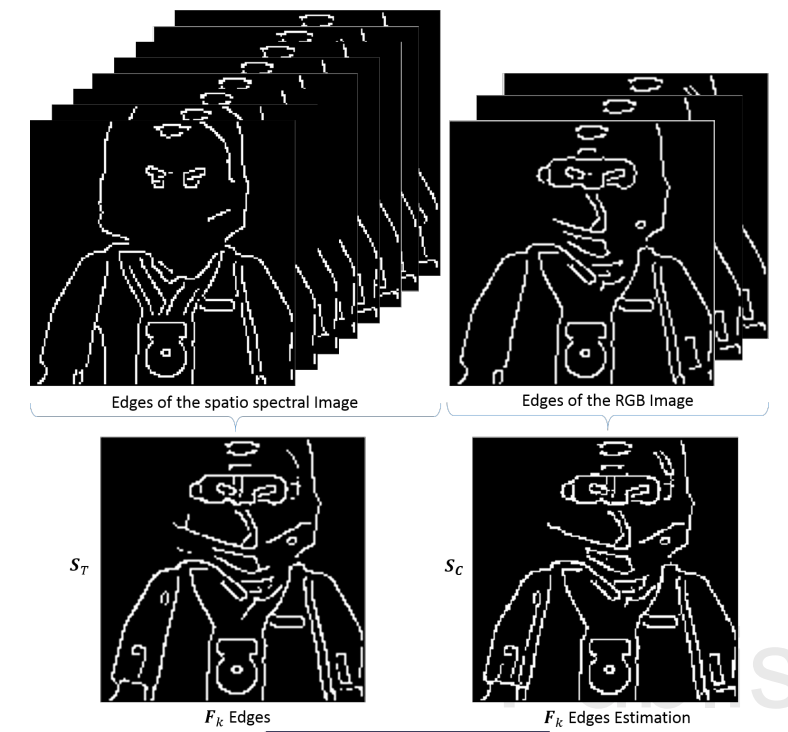
\includegraphics[width=300px]{edge_detection.png}
    \end{figure}
\end{center}
Note how the combination of the Random matrices and the edge detection matrices helps improving the density of pixels in areas of high frequencies.

Thus, by using this approach, we are optimizing the coded snapshot holes frequency to regions where it is needed to capture high frequency changes in the image. Hence, we get the sensing matrix. In the sample showed above, 87\% of the edges are correctly estimated from the RGB image. The details of these regions are well-preserved.


\subsection{Optimization Technique}

We finally have two measurements. One by the existing RGB code and the other by the freshly designed snapshot. The two measurements are stacked together onto a single vector. The equation is written as- $\tilde{y} = \tilde{H}f + \tilde{w} $, where all three of $\tilde{y}, \tilde{H}, \tilde{w}$ are the concatenated versions from the RGB and default sensor respectively.

The optimization is the following-
$$ \hat{f}=\Psi \lbrace \text{argmin}_\theta || \tilde{y} - \tilde{H}\Psi \theta ||_2 + \tau ||\theta||_1\rbrace $$

This is the familiar problem, which we have also seen in the class. The $\Psi$ is a bit different. To quote the paper
\begin{quotation}
    $\Phi$ is formulated as the Kronecker product of two bases $\Phi = \Phi_1 \otimes \Phi_2 $, where $\Phi_1$ is a 2D wavelet Symmlet 8 basis and $\Phi_2$ is playing the role of spectral sparsifier is a the 1D discrete cosine transform.
\end{quotation}

To solve this, the GSPR (gradient projection for sparse reconstruction) is used.

\subsection{Results}

Here is a sample sensing matrix of the following images-
\begin{center}
    \begin{figure}[!h]
        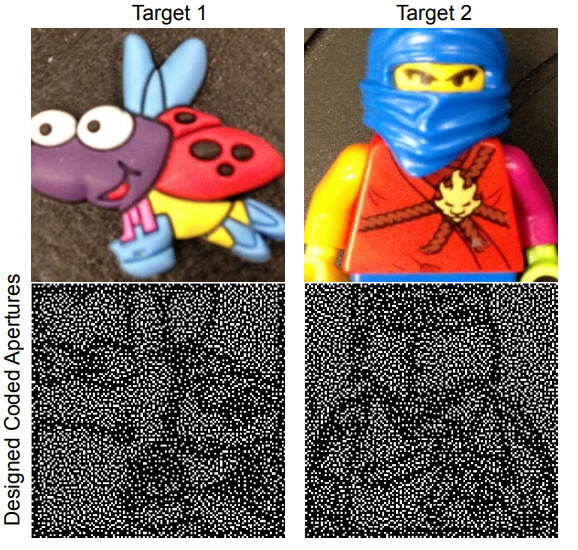
\includegraphics[width=300px]{designed_aperture.png}
    \end{figure}
\end{center}

The compressive sensing gradient projection for sparse reconstruction (GPSR) algorithm is used to obtain the reconstructions of the data cube. The reconstruction from this method have lesser noise and better information around edges. Here are some samples of the same-
\begin{center}
    \begin{figure}[!h]
        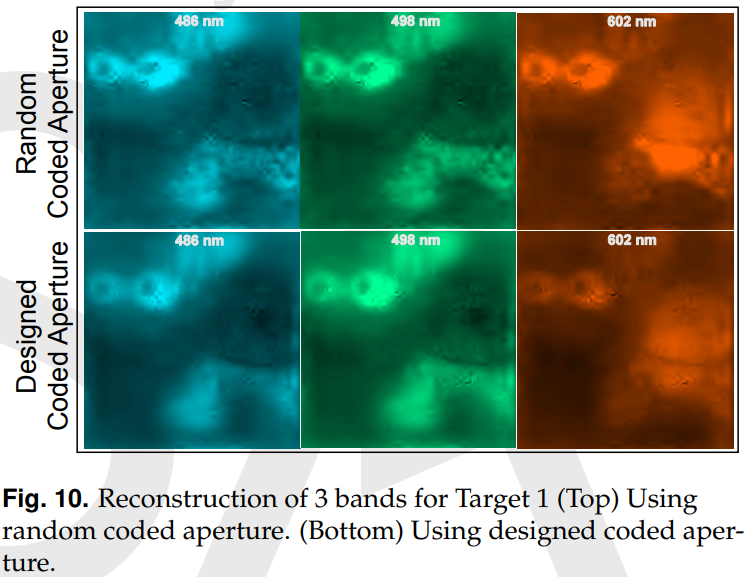
\includegraphics[width=250px]{sample_1.png}
    \end{figure}
\end{center}

We can see that the new method gives a much better Signal to Noise ratio, approximately a 3db improvement. Apart from this, due to better information of the active sights, the image is well lit as compared to random matrix.

Thus, we observe a higher intensity at high frequency points and a lower intensity at low frequency points, as is clear from the graph below. This is better for any image. Hence, this concludes our discussion of this architecture.

\begin{center}
    \begin{figure}[!h]
        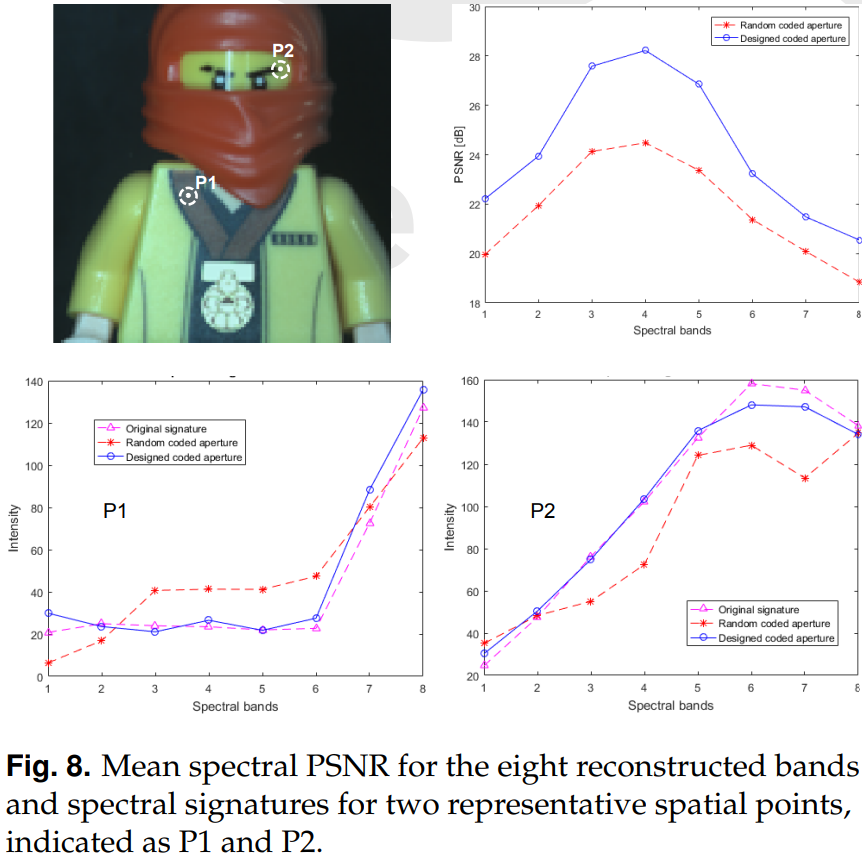
\includegraphics[width=250px]{sample_2.png}
    \end{figure}
\end{center}


\section{Problem 5}

Let
\begin{gather*}
    \boldsymbol{x^* := \mathrm{min}_{x\in\mathbb{K}^n}(\lVert y-\Phi x\rVert^2_2 + \lambda\lVert x\rVert_1)}\\
    \boldsymbol{\epsilon^{\prime} := \lVert y-\Phi x^*\rVert_2}\\
    \boldsymbol{A_t := \{x_0: x_0 \in \mathbb{K}^n;\;\lVert y-\Phi x_0\rVert_2\leq t\}}
\end{gather*}
Thus the sample space of the problem P1 for any given $\boldsymbol{\epsilon}$ is $\boldsymbol{A_{\epsilon}}$. Now, choose $\boldsymbol{\epsilon = \epsilon^{\prime}}$. Thus, $\boldsymbol{\lVert y-\Phi x\rVert_2 \leq \epsilon^{\prime}}$ $\forall$ $\boldsymbol{x\in A_{\epsilon^{\prime}}}$. But since the value of $\boldsymbol{\lVert y-\Phi x\rVert_2}$ over $\boldsymbol{A_{\epsilon^{\prime}}}$ is lesser than or equal to $\boldsymbol{\epsilon^{\prime}}$, we have that their L1 norms should be greater than or equal to $\boldsymbol{\lVert x^*\rVert_1}$ because otherwise if there existed $\boldsymbol{x^{\prime}\in A_{\epsilon^{\prime}}}$ such that $\boldsymbol{\lVert y-\Phi x^{\prime}\rVert_2 \leq \epsilon^{\prime}}$ and $\boldsymbol{\lVert x^{\prime}\rVert_1 < \lVert x^*\rVert_1}$, then $\boldsymbol{J(x^{\prime}) < J(x^*)}$, contradicting the minimality of $\boldsymbol{x^*}$.

Thus $\boldsymbol{\lVert x^{\prime}\rVert_1 \geq \lVert x^{*}\rVert_1}$ $\forall$ $\boldsymbol{x^{\prime}\in A_{\epsilon^{\prime}}}$ (note that $\boldsymbol{x^*\in A_{\epsilon^{\prime}}}$ too). Thus, the set of vectors with minimum L1-norms in $\boldsymbol{A_{\epsilon^{\prime}}}$ includes $\boldsymbol{x^*}$, and consequently $\boldsymbol{x^*}$ is a minimizer for problem P1 too (although note that without additional information we can't say if $\boldsymbol{x^*}$ is the unique minimizer of P1 or not).


\section{Problem 6}
We use the linearity of expectation to find out the number of tests. Thus, the expected number of tests required for the entire population is equal to the
(Number of groups) multiplied by the expected number of tests required for a single group.

Now, let $p = \frac{k}{n}$ be the probability that a randomly chosen person is infected. Then, the expected number of tests that need to be carried out can be calculated as follows:

\begin{itemize}
    \item Suppose none of our $g$ pool members are infected. The probability of this happening is $(1-p)^g$, and thus the contribution of this scenario to the expected value is $(1-p)^g\cdot 1$, ie:- after carrying out the initial pool test itself we can declare all of the pool members to be negative.
    \item Suppose at least one of our pool members is infected. The probability of this happening is $1-(1-p)^g$, and in this case we need to carry out $(g+1)$ tests according to the Dorfman algorithm (one initial pool test, and then $g$ individual tests). Thus, the contribution of this scenario to the expected value is $(1-(1-p)^g)\cdot (g+1)$.
\end{itemize}

Thus the total expected value of the number of tests that need to be carried out for a single pool is $(1-p)^g + (1-(1-p)^g)\cdot (g+1) = 1 + g(1-(1-p)^g)$, and consequently the \textbf{number of tests required for the entire population is} $\frac{n}{g}\cdot (1 + g(1-(1-p)^g)) = \boldsymbol{\frac{n}{g} + n(1-(1-p)^g)}$, where $p = \frac{k}{n}$.\\
Now, coming to the worst case, the worst case will occur when all the $k$ patients land up in different groups: In that case, firstly in the $\frac{n}{g}$ group tests, $k$ groups will come out to be positive, and then all patients among those $k$ groups have to be tested to determine the actual patients.

\textbf{Thus the number of tests required in the worst case is $\boldsymbol{\frac{n}{g} + kg}$}.

% For simplifying our further calculations, we shall assume that $p = \frac{k}{n} \ll 1$ is a very small number and hence the binomial approximation is applicable on $(1-p)^g$, which yields $(1-p)^g\approx 1-gp$, and consequently the expected value of the number of tests that need to be carried out becomes $\approx (\frac{n}{g} + ngp) = n\cdot (\frac{1}{g} + gp)$. Minimizing this expression w.r.t $g$ to obtain the optimal group size yields $\frac{1}{(g^*)^2} = p\Rightarrow g^* = \frac{1}{\sqrt{p}} = \frac{1}{\sqrt{k/n}} = \sqrt{\frac{n}{k}}$, ie:- the \textbf{optimal group size is $\boldsymbol{\sqrt{\frac{n}{k}}}$, where $k$ is the number of people infected and $n$ is the population size}.

Now, to minimize the number of tests required even for the worst case, we differentiate w.r.t $g$ to get that $\frac{1}{(g^*)^2} = \frac{k}{n}\Rightarrow g^* = \frac{1}{\sqrt{k/n}} = \sqrt{\frac{n}{k}}$, ie:- the \textbf{optimal group size in the worst case is $\boldsymbol{\sqrt{\frac{n}{k}}}$, where $k$ is the number of people infected and $n$ is the population size}.













\end{document}

From the theory of \textbf{Singular Value Decomposition} we know that the singular values of any matrix $A$ are the \textbf{square roots of the eigenvalues of $\boldsymbol{AA^*}$} (note that the eigenvalues of $\boldsymbol{AA^*}$ are non-negative by the Spectral theorem since $\boldsymbol{AA^*}$ is Hermitian). Thus, to calculate the singular values of $\boldsymbol{\Phi_S^{\dagger}}$, we first evaluate the matrix $\boldsymbol{\Phi_S^{\dagger}}\boldsymbol{\Phi_S^{\dagger^{*}}}$ 
$$\boldsymbol{\Phi_S^{\dagger}\Phi_S^{\dagger^{*}} = ((\Phi_S^*\Phi_S)^{-1}\Phi_S)(\Phi_S^*(\Phi_S^*\Phi_S)^{-1}) = (\Phi_S^*\Phi_S)^{-1}}$$
Thus, $\boldsymbol{\Phi_S^{\dagger}\Phi_S^{\dagger^{*}} = (\Phi_S^*\Phi_S)^{-1}}$. Now, we utilise a linear algebra property which says that if $\lambda$ is an eigenvalue of an invertible matrix $A$, then $\frac{1}{\lambda}$ will be an eigenvalue of the matrix $A^{-1}$. \\
Since $\boldsymbol{\Phi_S^*\Phi_S}$ is obviously invertible, the eigenvalues of $\boldsymbol{(\Phi_S^*\Phi_S)^{-1}}$ are the reciprocals of the eigenvalues of $\boldsymbol{\Phi_S^*\Phi_S}$.\\
Now, since $\boldsymbol{\Phi}$ is RIC with order $|S| = 2k$, from the slides (\texttt{CS\_Theory, Pg.101/109}) we have that $\boldsymbol{\delta_{2k}}$ = max$\boldsymbol{(\lambda_{\mathrm{max}}-1, 1-\lambda_{\mathrm{min}})}$ where $\boldsymbol{\lambda_{\mathrm{max}}}$ is the maximum eigenvalue of $\boldsymbol{\Phi_{\Gamma}\Phi_{\Gamma}^*}$ and $\boldsymbol{\lambda_{\mathrm{min}}}$ is the minimum eigenvalue of $\boldsymbol{\Phi_{\Gamma}\Phi_{\Gamma}^*}$ over all possible sets $\boldsymbol{\Gamma\subseteq[n],\;|\Gamma| \leq |S|}$ (note that $\boldsymbol{\lambda_{\mathrm{max}}}$ and $\boldsymbol{\lambda_{\mathrm{min}}}$ both don't necessarily come from some same set $\boldsymbol{\Gamma}$). Then, considering the fact that $\boldsymbol{\Phi_{\Gamma}\Phi_{\Gamma}^*}$ and $\boldsymbol{\Phi_{\Gamma}^*\Phi_{\Gamma}}$ have the same non-zero eigenvalues (this is again a linear algebra property: For any matrix $A$, $\boldsymbol{AA^*}$ and $\boldsymbol{A^*A}$ have the same non zero eigenvalues), we see that every eigenvalue of $\boldsymbol{\Phi_S^*\Phi_S}$ lies in $\boldsymbol{[1-\delta_{2k}, 1+\delta_{2k}]}$ (because note that $S$ is just an instance of $\boldsymbol{\Gamma}$ and  $\boldsymbol{\delta_{2k}}$ = max$\boldsymbol{(\lambda_{\mathrm{max}}-1, 1-\lambda_{\mathrm{min}})}$ implies that all eigenvalues, are first bounded by $\boldsymbol{\lambda_{\mathrm{max}}}$ and $\boldsymbol{\lambda_{\mathrm{min}}}$ which are in turn bounded by $\boldsymbol{1-\delta_{2k}}$ and $\boldsymbol{1+\delta_{2k}}$. Refer to the solution of Q3 for an elaboration of the same), and consequently \textbf{EVERY} singular value of $\boldsymbol{\Phi_S^{\dagger}}$, which as we showed above were the square roots of the reciprocals of the eigenvalues of $\boldsymbol{\Phi_S^*\Phi_S}$, must lie within $\boldsymbol{[\frac{1}{\sqrt{1+\delta_{2k}}}, \frac{1}{\sqrt{1-\delta_{2k}}}]}$, as desired.